\documentclass[a4paper,11pt]{article}
\usepackage[latin1]{inputenc}
\usepackage[T1]{fontenc}
\usepackage{amsmath}
\usepackage{a4wide}
\usepackage{booktabs}
\usepackage{graphicx}
\usepackage{url}

\title{Genomics and Bioinformatics}
\date{October 29, 2013}
\author{Exam correction}
\begin{document}
\maketitle

\section*{Question 1 - Genome Assembly}

\begin{enumerate}

\item
\begin{figure}[h]
\centering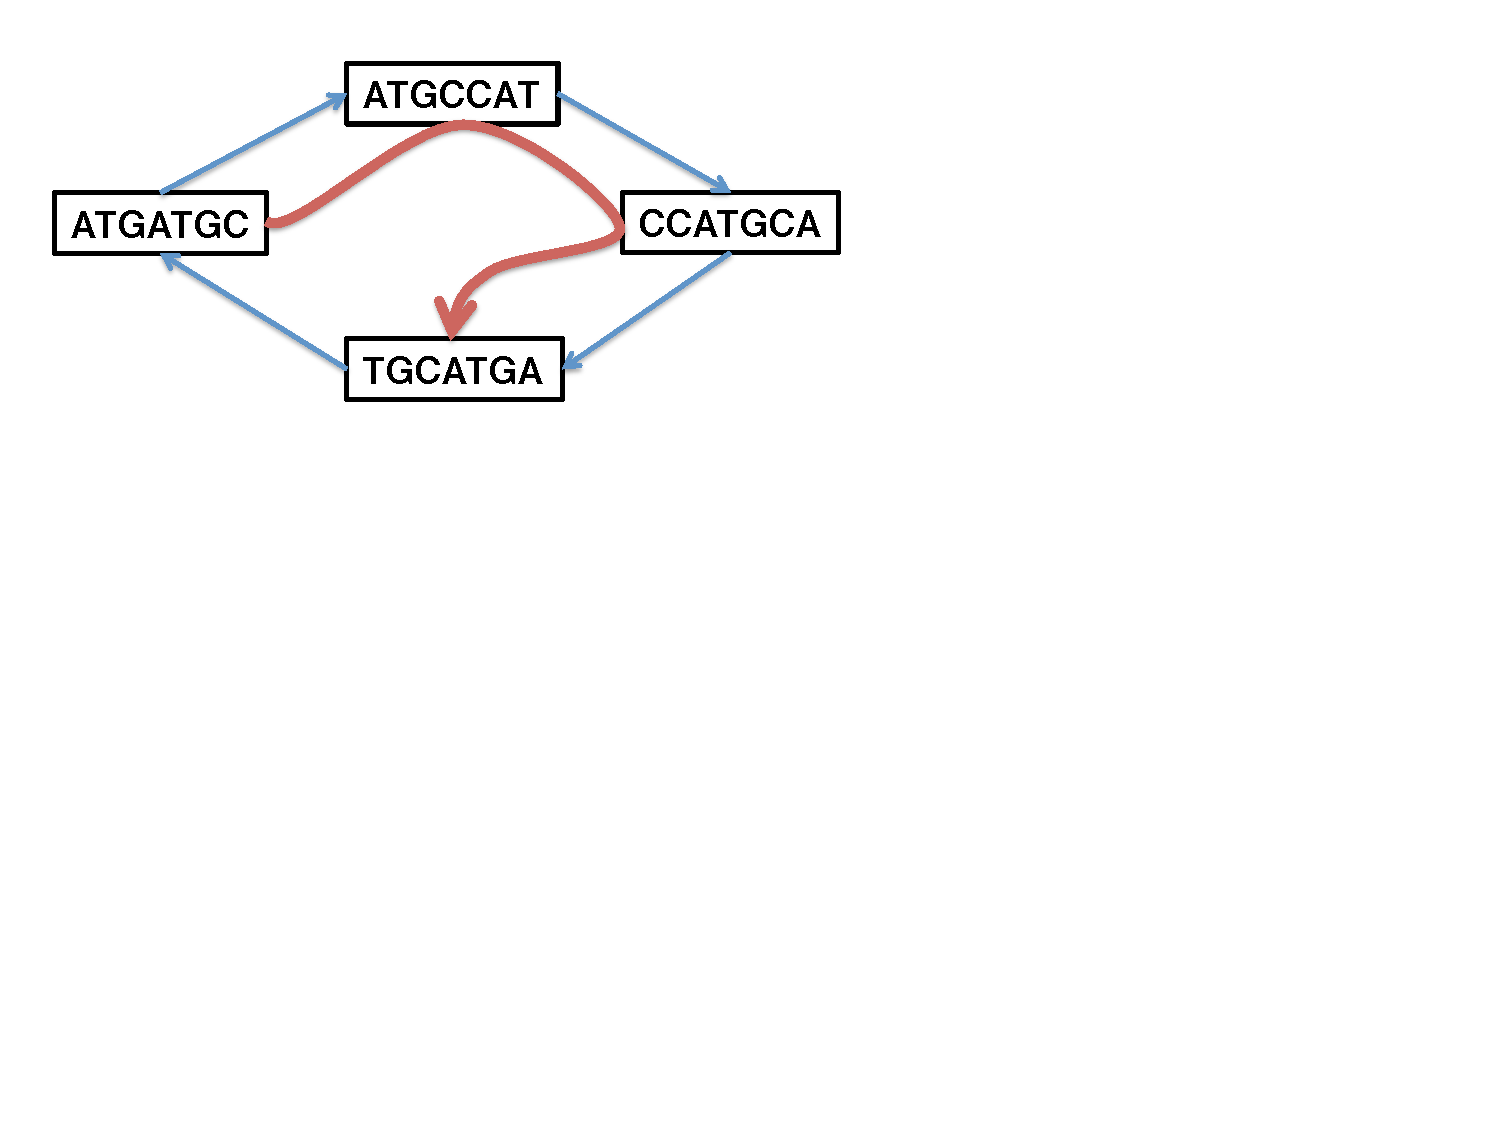
\includegraphics[scale=.8]{Hamilton.pdf}
\end{figure}

A Hamiltonian path follows the red arrow and generates the
following contig:\\
\textbf{ATGATGCCATGCATGA}

\item 
The 4-mers and 5-mers sets are:
\begin{eqnarray*}
  S_4 &=& \{\mbox{\bf ATGA, TGAT, GATG, ATGC, TGCC,} \\
  &&\phantom\{\mbox{\bf GCCA, CCAT, CATG, TGCA, GCAT}\}.\\
  S_5&=&\{\mbox{\bf ATGAT, TGATG, GATGC, ATGCC, TGCCA, GCCAT,} \\
  &&\phantom\{\mbox{\bf CCATG, CATGC, ATGCA, TGCAT, GCATG, CATGA}\}.
\end{eqnarray*}


\item The de Bruijn graph is as below:
\begin{figure}[h]
\centering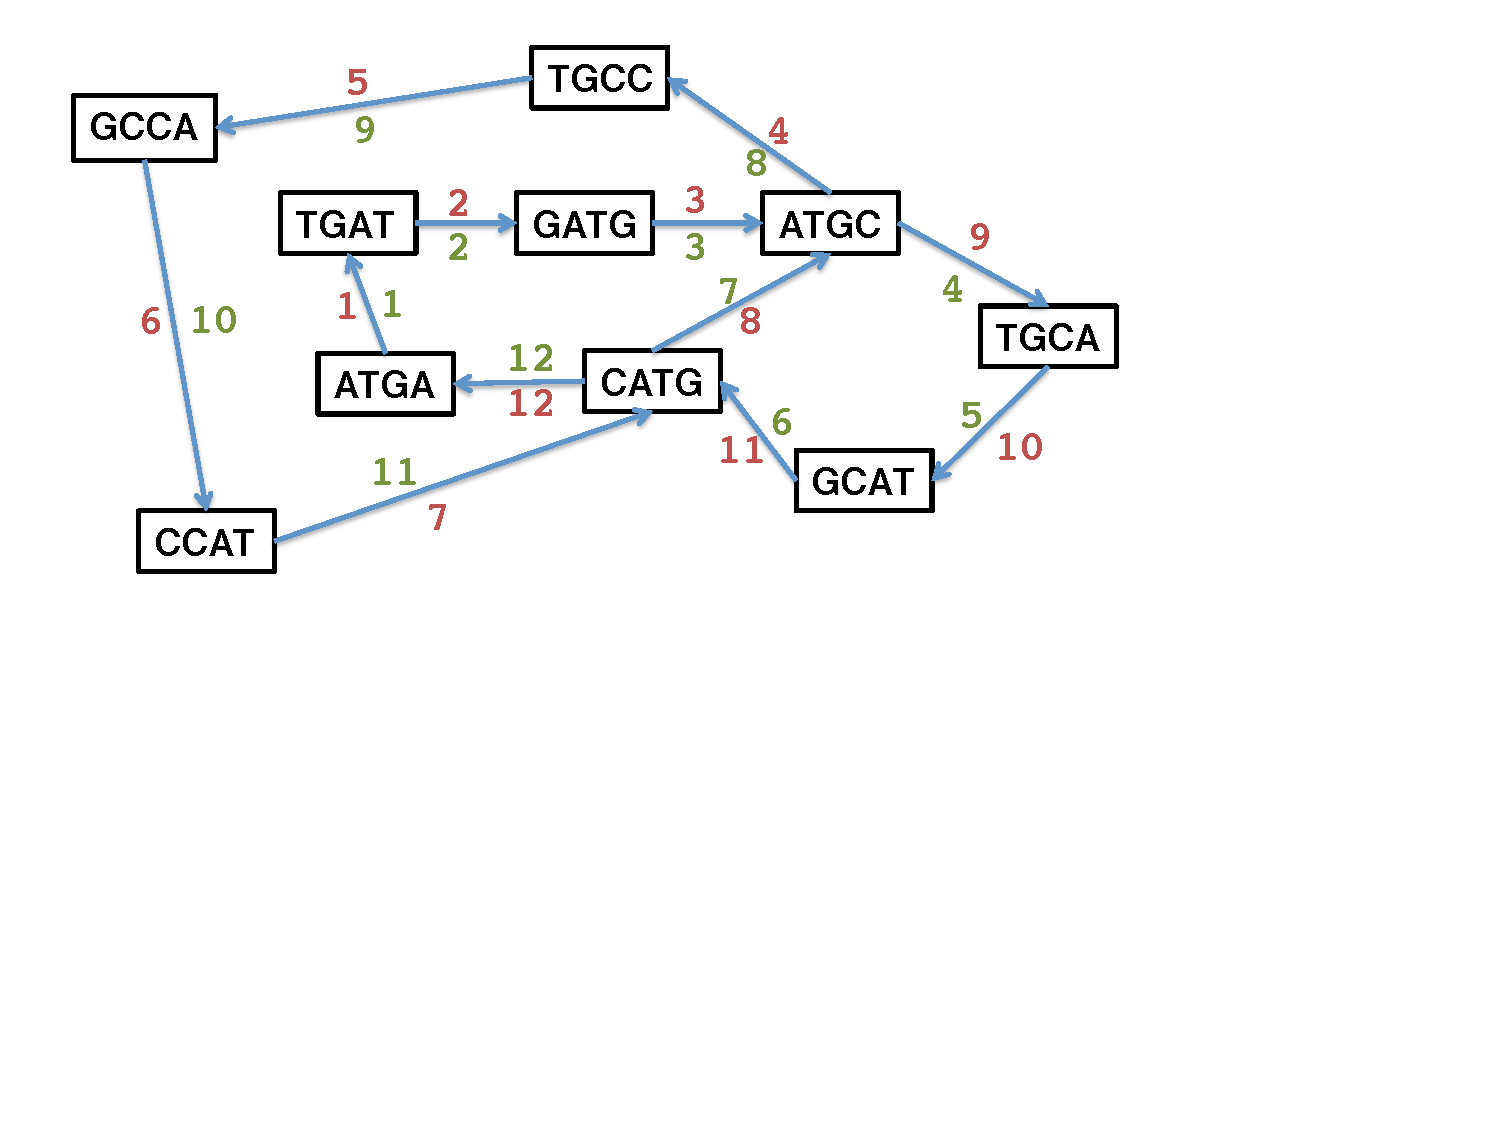
\includegraphics[scale=.8]{Bruijn.pdf}
\end{figure}

\item This graph is Eulerian: for every vertex the number of
  incoming edges is always equal to the number of outgoing edges.

\item 
One eulerian path follows the edges in the order of the red numbers
and generates the contig\\
\textbf{ATGATGCCATGCATGA}\\
and the green numbering leads to\\
\textbf{ATGATGCATGCCATGA}\\

The second contig could not have generated the reads \textbf{CCATGCA}
and \textbf{TGCATGA}.
\end{enumerate}


\section*{Question 2 - Sequence Alignment}

\subsection*{Linear gap penalty}

\begin{figure}[h]
\centering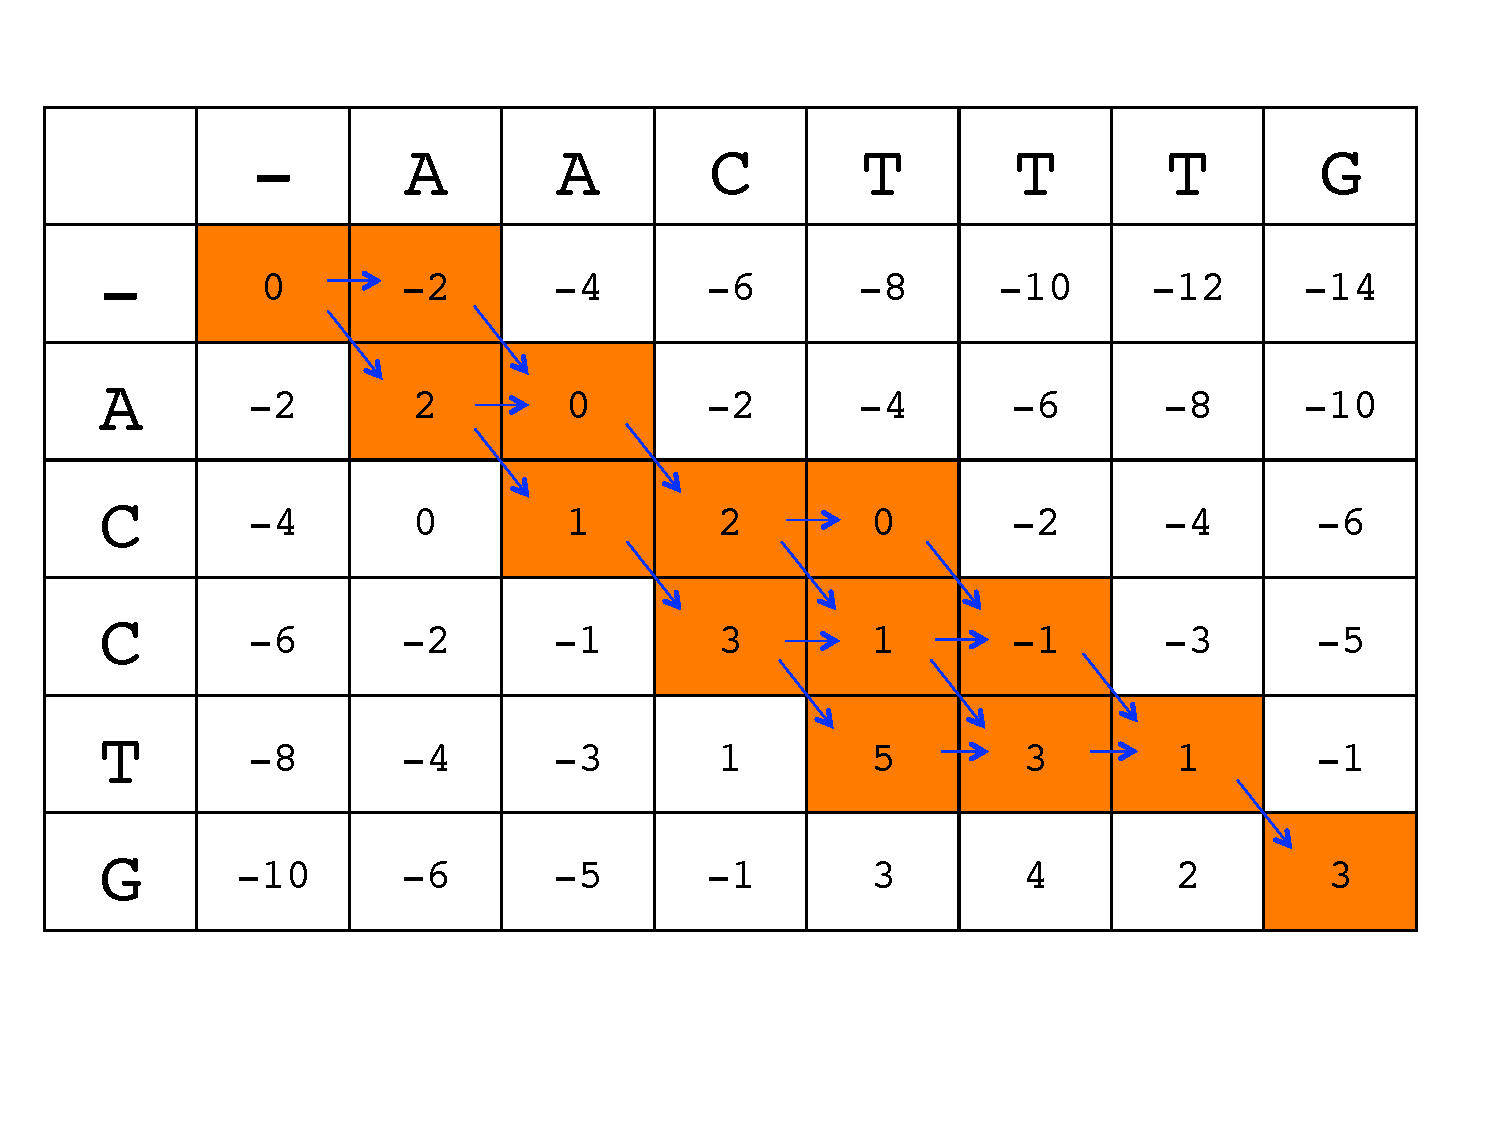
\includegraphics[scale=.4]{scoring_matrix.pdf}
\end{figure}

\noindent The nine optimal alignments have score = 3 and are given as follows:

\begin{verbatim}
AACTTTG  AACTTTG  AACTTTG  AACTTTG  AACTTTG  AACTTTG  AACTTTG  AACTTTG  AACTTTG
ACCT--G  ACC--TG  ACC-T-G  -ACCT-G  -AC-CTG  -ACC-TG  A-CCT-G  A-C-CTG  A-CC-TG

\end{verbatim}

\subsection*{Affine gap penalty}

The first two alignments have $1$ gap opening, so their score is 
$$
3 - 1 \times 2 \,=\, 1~.
$$
All the others have $2$ gap openings, so a score of
$$
3-2\times 2\,=-\,1~.
$$

\section*{Question 3 - Hidden Markov Model}

\begin{enumerate}

\item Let us call $T$ a transmembrane domain, $E$ an extracellular
  domain, $I$ an intracelular domain: these are the hidden states.
The simplest diagram is as follows:
\begin{figure}[h]
\center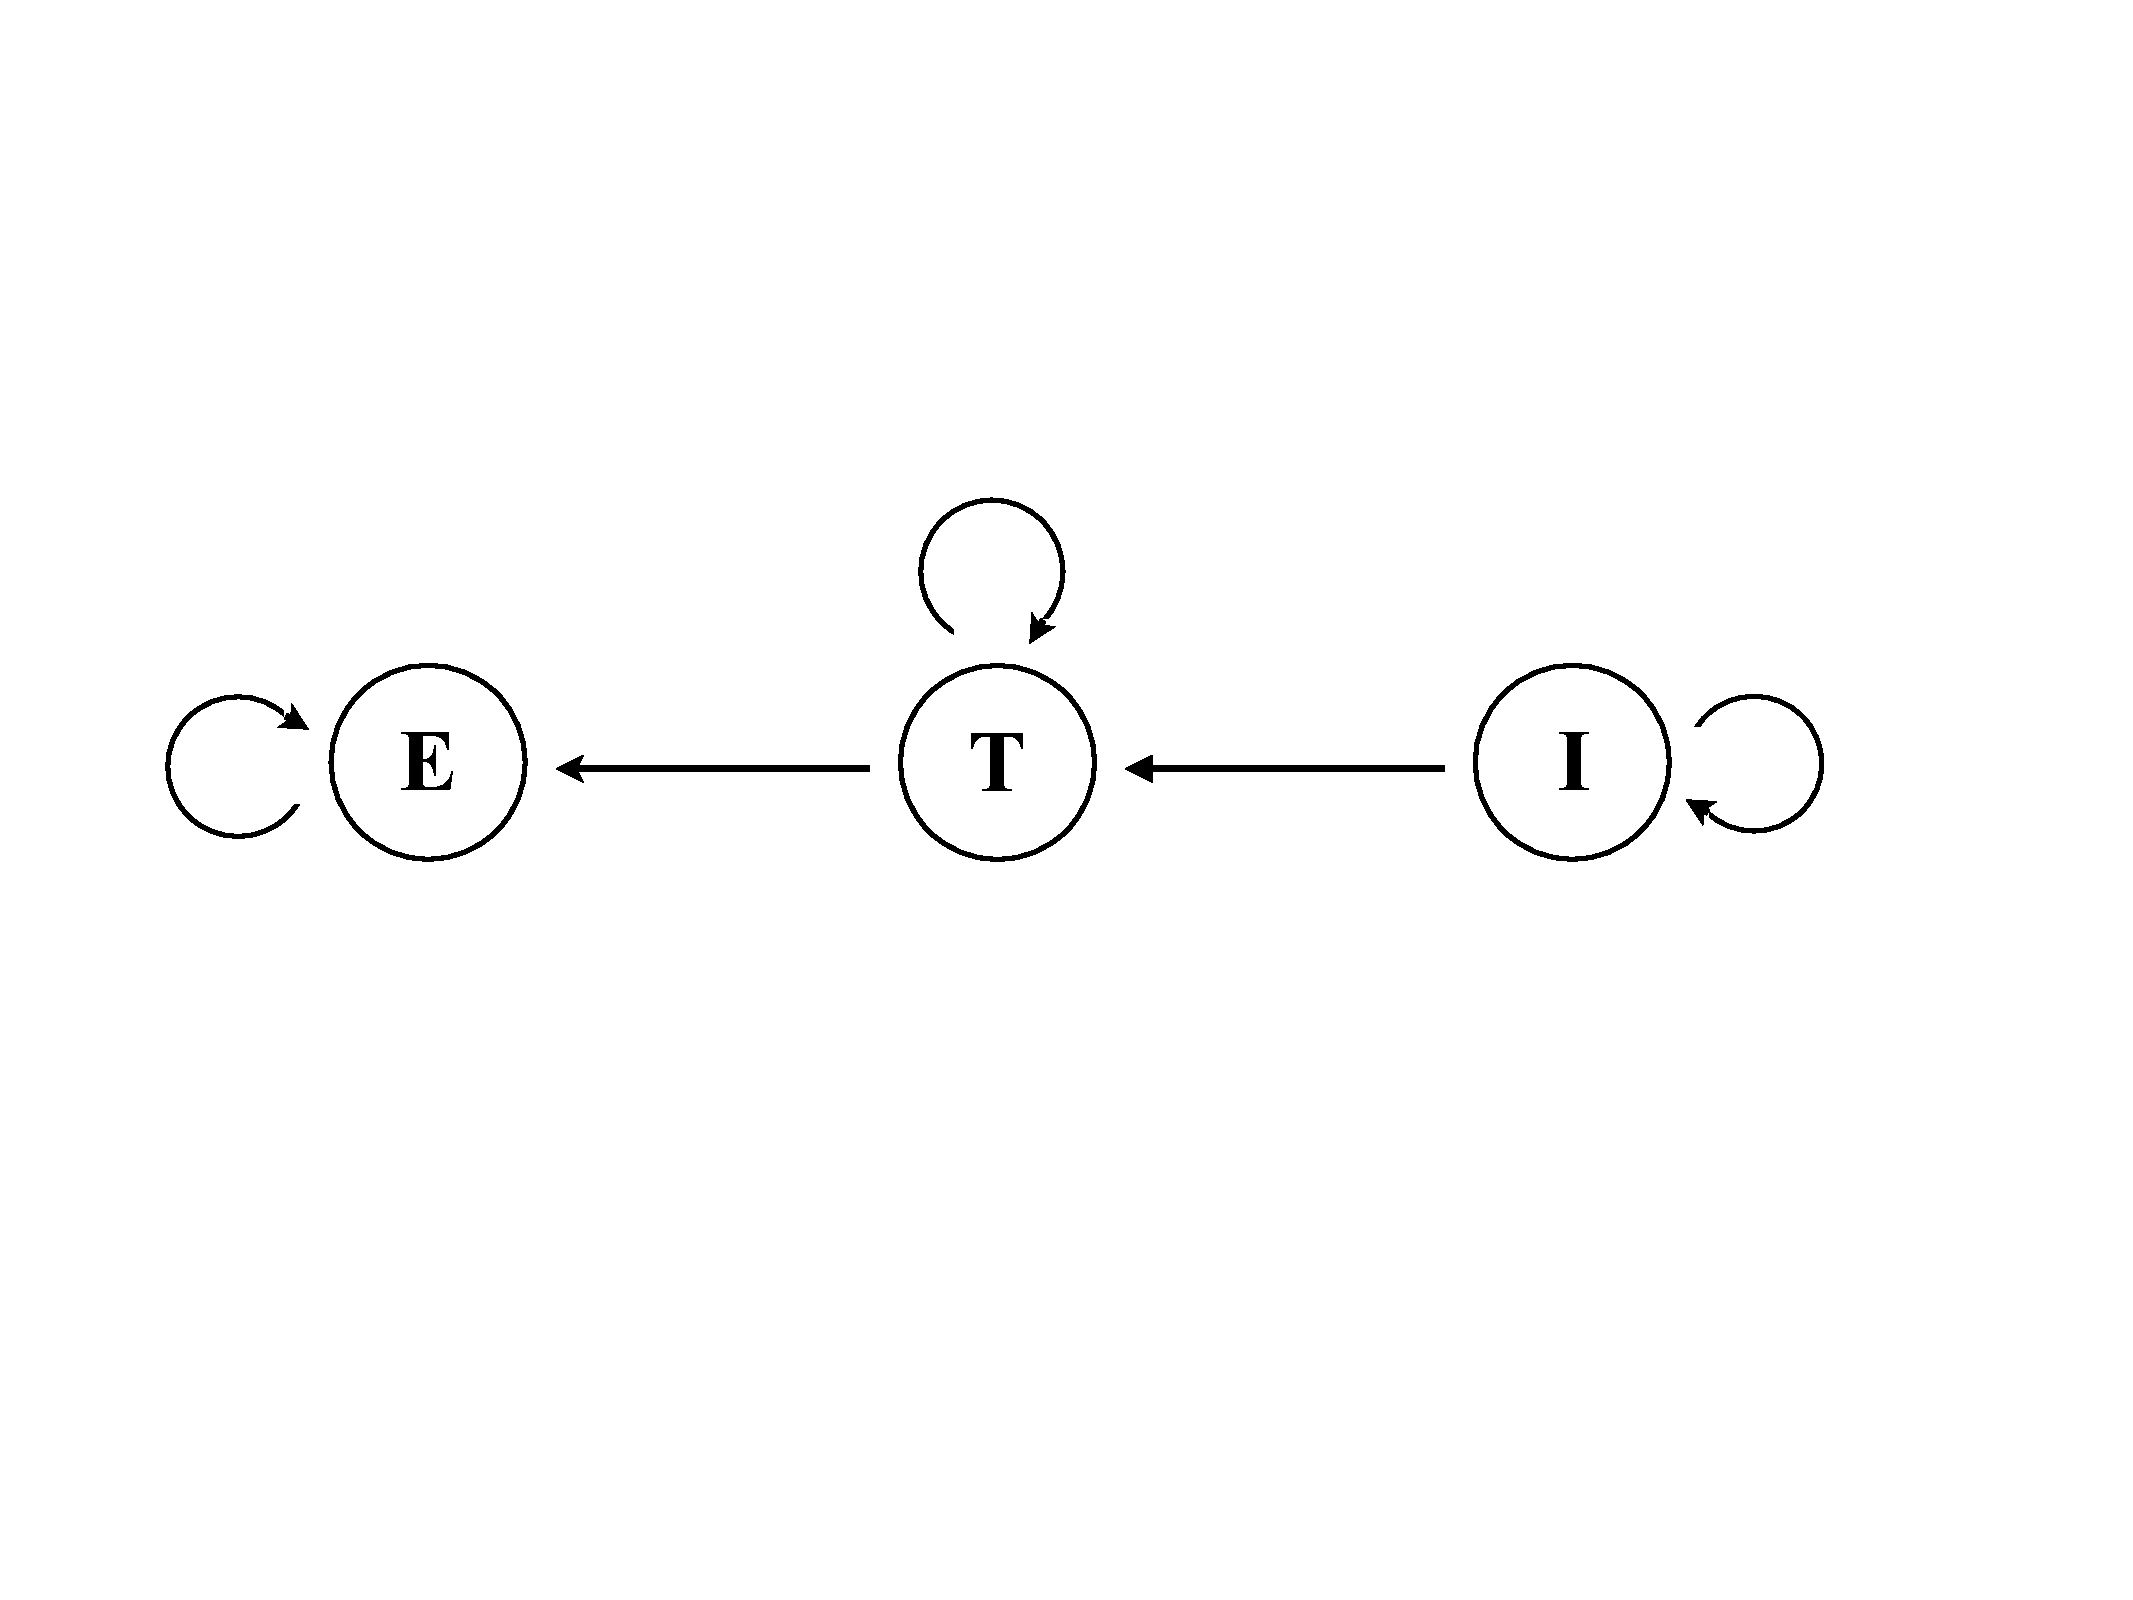
\includegraphics[scale=.4]{hmm_graph1.pdf}
\end{figure}

but this doesn't allow more than one transmembrane domain.
One could add reverse arrows, but then it would allow $I\rightarrow T \rightarrow I$ transitions.
To accomodate several transmembrane domains we can 
use two identical states $T1$ and $T2$: 
\begin{figure}[hbt]
\center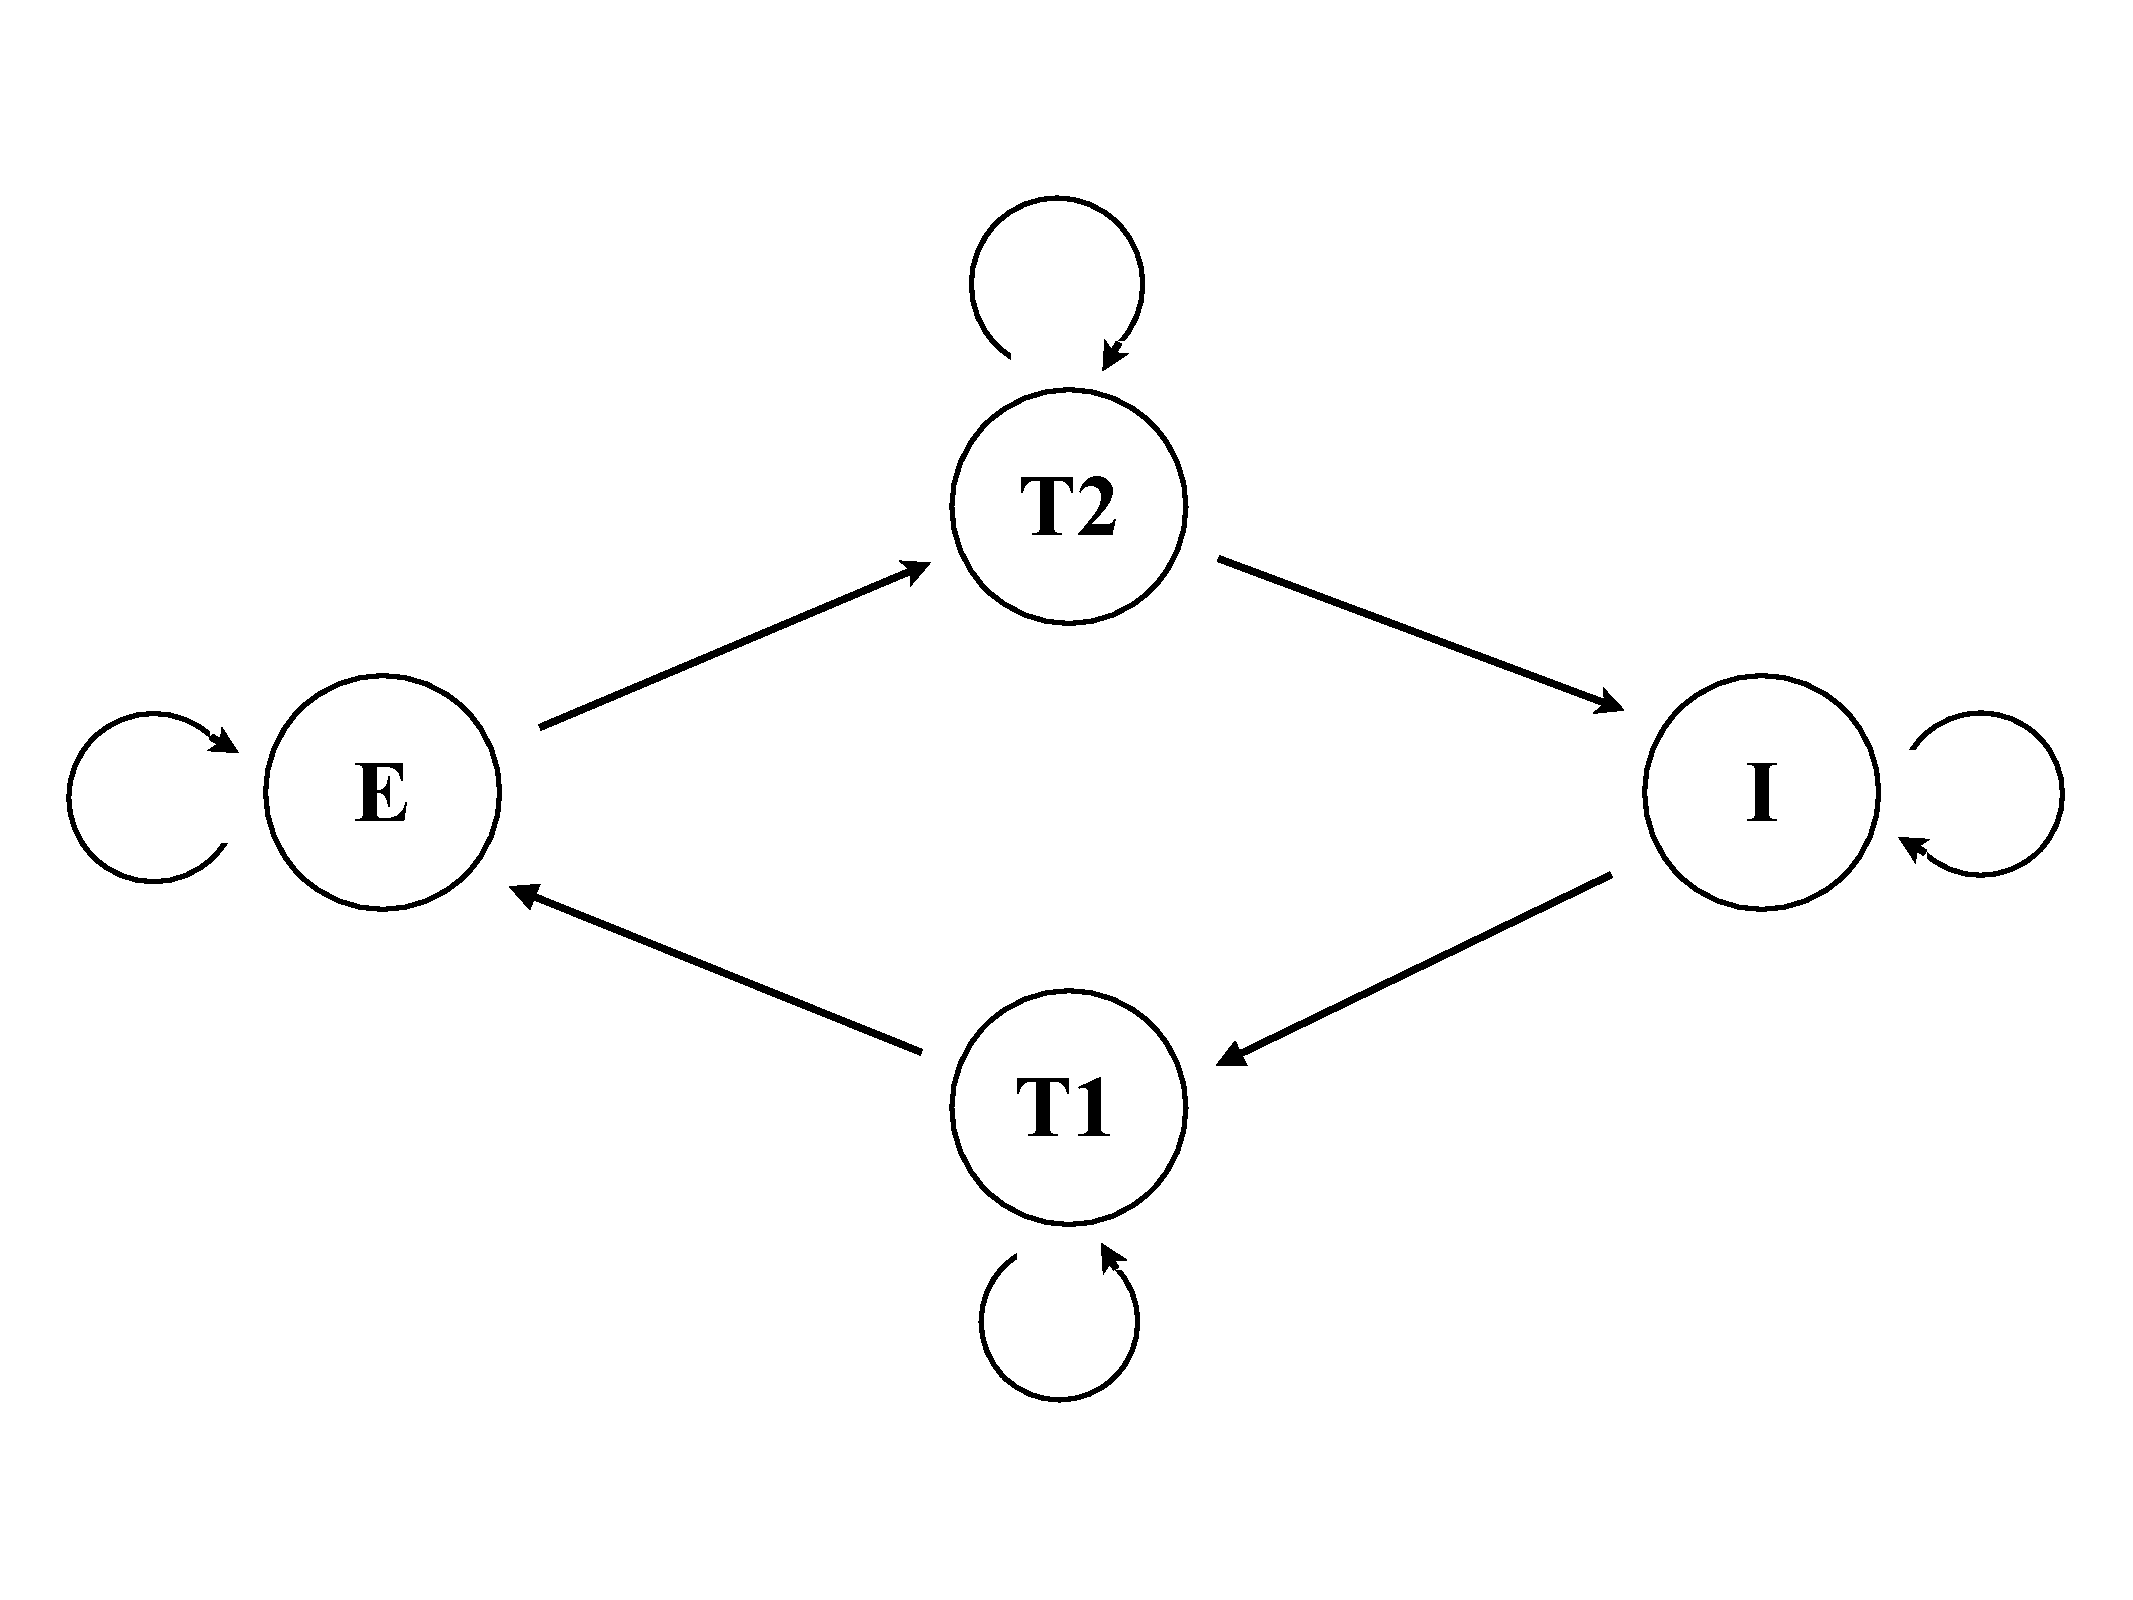
\includegraphics[scale=.4]{hmm_graph2.pdf}
\end{figure}

There may be other models, but we give the solution only for these two.

\item The emissions from the $T$ state are given by the helical
  propensity table. 
In other domains, since all amino-acids are equiprobable, 
each has a frequency $1/20=5\%$.

\item As we saw in an earlier exercise, the transition probabilities
  can be set as the inverse of the expected segment length.
In this case, there are about 20 amino-acids in a transmembrane domain, so we can set the probability of
going out of T as $1/20$.

If we use two $T$ states, $T1\rightarrow E$ and $T2\rightarrow I$
transitions both have probability $1/20$.
Outgoing probabilities must sum to $1$, so the transition $T\rightarrow T$ is $19/20$. 

In the $E$ state, the outgoing probability is $1/400$ (therefore $E\rightarrow E$ is 
$399/400$) and similarly for $I$ we have $1/200$ and $199/200$. This
yields the following transition matrices:
$$
\begin{array}{c}
E \\ T_2 \\ I \\ T_1
\end{array}
\left( 
\begin{array}{cccc}
399/400 & 1/400 & 0            & 0 \\
0            & 19/20 & 1/20       & 0 \\
0            & 0        & 199/200 & 1/200 \\
1/20       & 0        & 0            & 19/20 \\
\end{array}
\right)
\quad \mbox{or} \quad 
\begin{array}{c}
E \\ T \\ I
\end{array}
\left( 
\begin{array}{ccc}
1 & 0 & 0 \\
1/20       & 19/20 & 0 \\
0            & 1/200 & 199/200 
\end{array}
\right)~.
$$

One can also use $1/201$, $200/201$, etc. as seen in the exercise. 

\item Use the Forward algorithm to compute the total probability of
  the observed sequence.

\item If $O_n$ is the $n$-th observation and $S_n$ is the $n$-th
  hidden state, we can write 
$$
P(O|S)
\, =\, P(O_1O_2O_3\dots | S_1S_2S_3\dots)
\, =\, P(O_1|S_1)\cdot P(O_2|S_2)\cdot P(O_3|S_3)\cdot \dots~.
$$
Emissions are equally probable in states $E$ and $I$: $P(O_1|S_1) =
P(N|E) = 5\%$ \textit{etc.}, and in the $T$ state we have
$P(O_3|S_3) = P(A|T) = 8\%$ and $P(O_4|S_4) = P(K|T) = 6\%$.
Finally:
$$
P(O|S)\, = \,(5\cdot 5\cdot 8\cdot 6\cdot 5\cdot 5\cdot 5) / 100^{7}\,
=\, \bf{1.5\cdot 10^{-9}}~.
$$

\textbf{\textit{Alternatively:}} One could also understand the question as finding $P(O,S)$ instead of $P(O|S)$, in which case 
we have $P(O,S) = P(O|S)\cdot P(S) $. We need 
$$
P(S) = P(S_1|S)\cdot P(S_2|S) ... = P(\text{initial state is } S_1)\cdot P(S_2|S_1) \cdot P(S_3|S_2)\cdot ...  
$$
which are the transition probabilities. Multiply that with the $P(O|S)$ from above. This version requires to choose
in which domain you start ($E$ or $I$). For instance, starting from $I$ and using the unidirectional 3-states model,
the known hidden sequence is $IITTEEE$ and we have:
$$
P(O,S) = \,1.5\cdot 10^{-9}\; \cdot \; (1\cdot \frac{199}{200}\cdot \frac{1}{200}\cdot \frac{19}{20}\cdot \frac{1}{20}
\cdot \frac{399}{400}\cdot \frac{399}{400})
$$

\item If transmembrane domains always contain a multiple of 4 amino-acids, one can extend the model as in the figure below.
Another solution would be to emit quadruplets of amino-acids when in state $T$, each with its specific probability.

\begin{figure}[hbt]
\centering
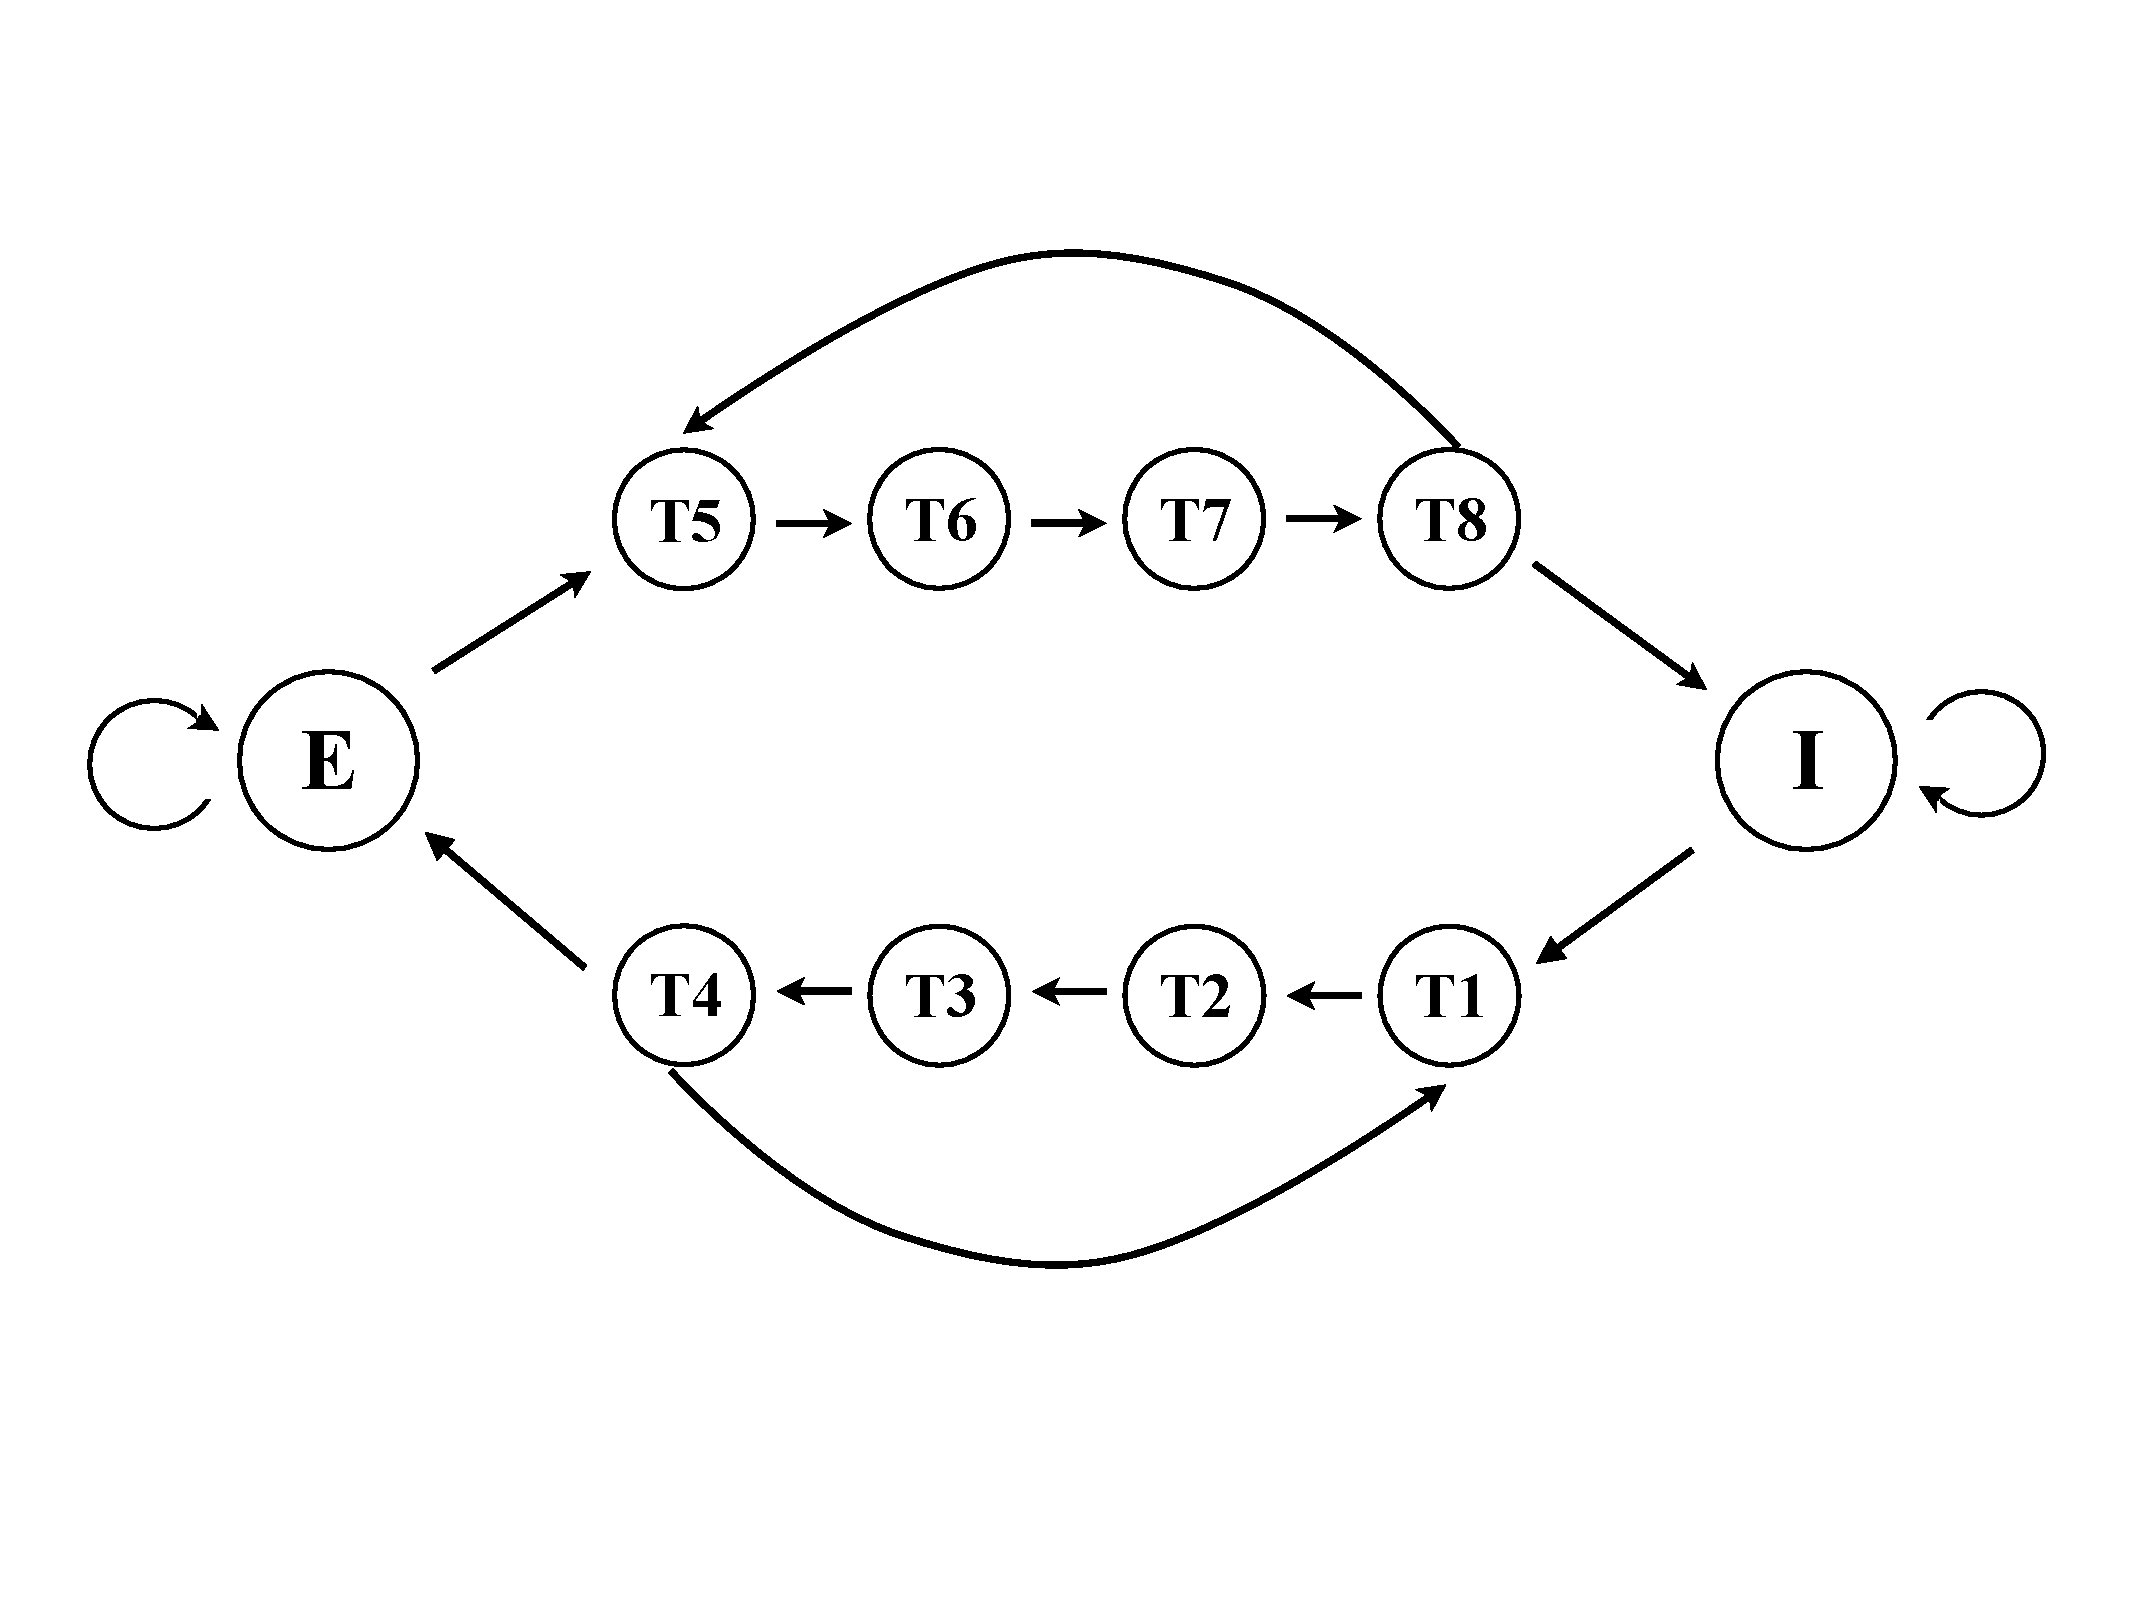
\includegraphics[width=0.6\textwidth]{hmm_graph3.pdf}
\end{figure}

\end{enumerate}

\pagebreak

\section*{Question 4 - Homology}

\begin{enumerate}
\item The tree below is compatible with the similarity scores. The red
  dot is a gene duplication, the green, blue and orange dots denote
  three speciation events.

\begin{figure}[h]
\centering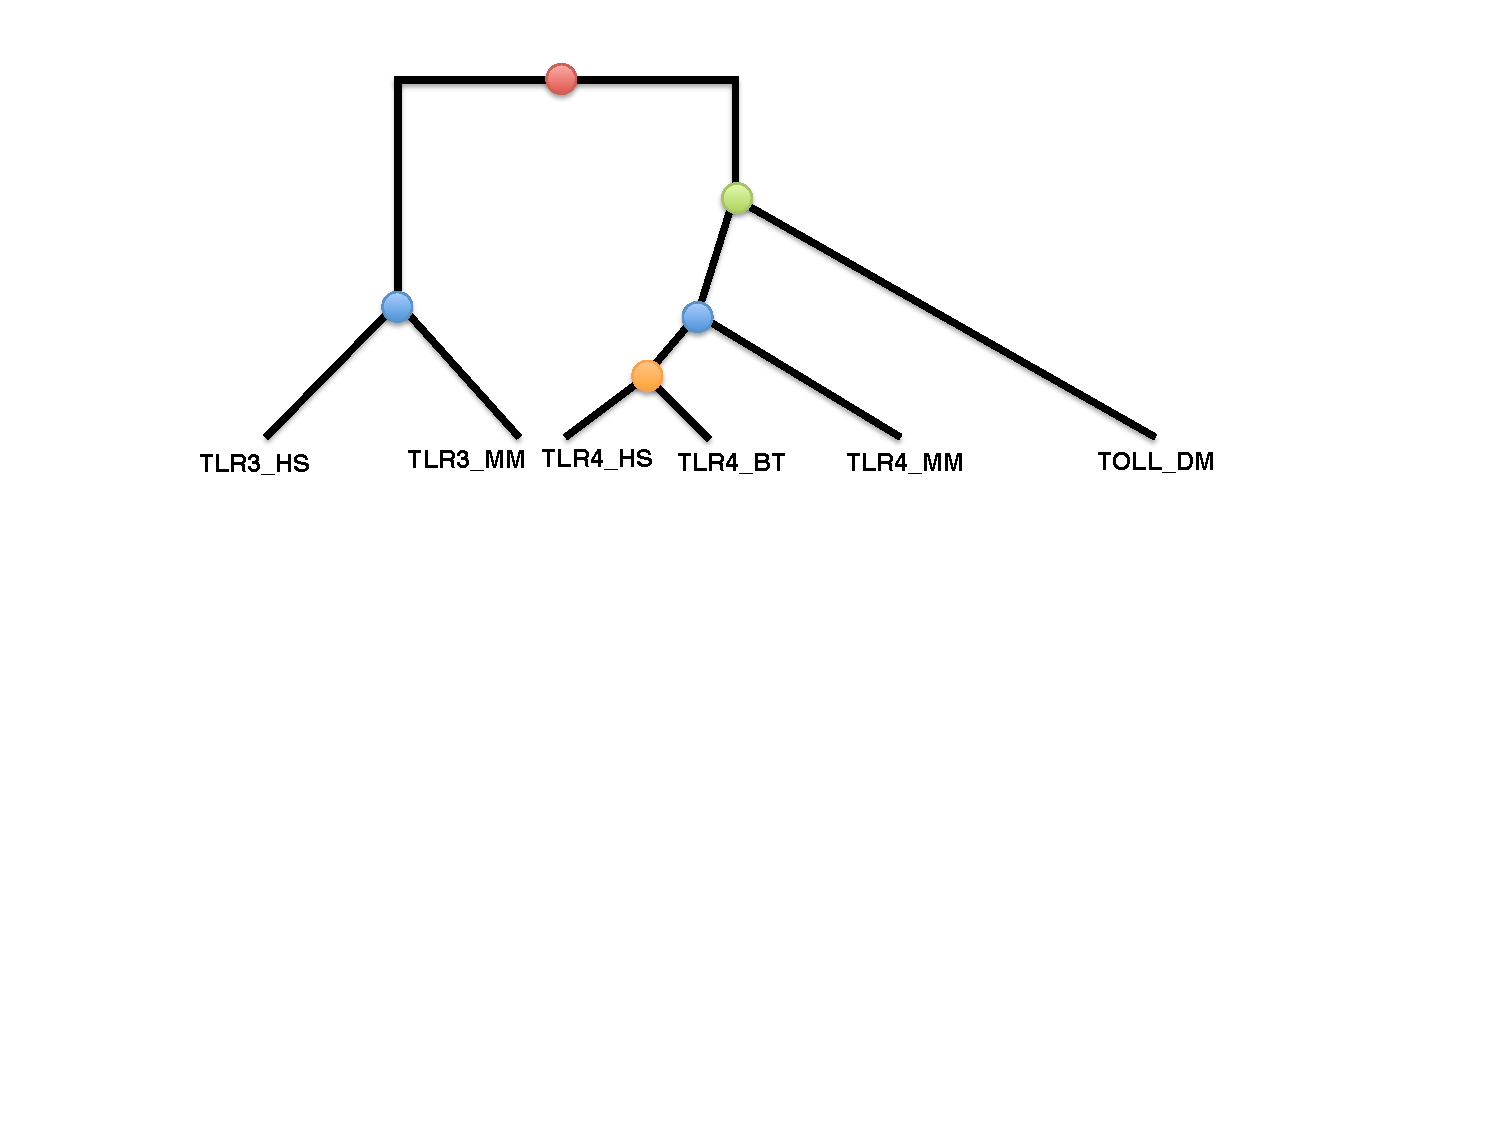
\includegraphics[scale=.6]{TreeSolution.pdf}
\end{figure}




\item Orthologous pairs:\\
  \item \textbf{TLR3\_HS} and \textbf{TLR3\_MM}, any combination of
    \textbf{TLR4\_MM}, \textbf{TLR4\_HS}, \textbf{TLR4\_BT} and \textbf{TOLL\_DM}.
\item Paralogous pairs in the same species:\\
\textbf{TLR3\_HS} and \textbf{TLR4\_HS}, \textbf{TLR3\_MM} and \textbf{TLR4\_MM}.
\item Paralogous pairs in different species:\\
\textbf{TLR3\_HS} or \textbf{TLR3\_MM} with any other protein in a
different species.
\end{enumerate}



\end{document}
